\subsection{Hybrides Vorgehen im Projekt}

Während die Stacey Matrix hilft das Projekt zu beurteilen und eine Entscheidung für klassisches oder agiles Vorgehen im Projekt zu treffen, gibt es andere Methoden und Hilfsmittel, den Projektkontext, nicht das Projekt als solches zu betrachten und einzuordnen. Eines davon ist das Agilometer:\\

\begin{figure}[hbt!]
\centering
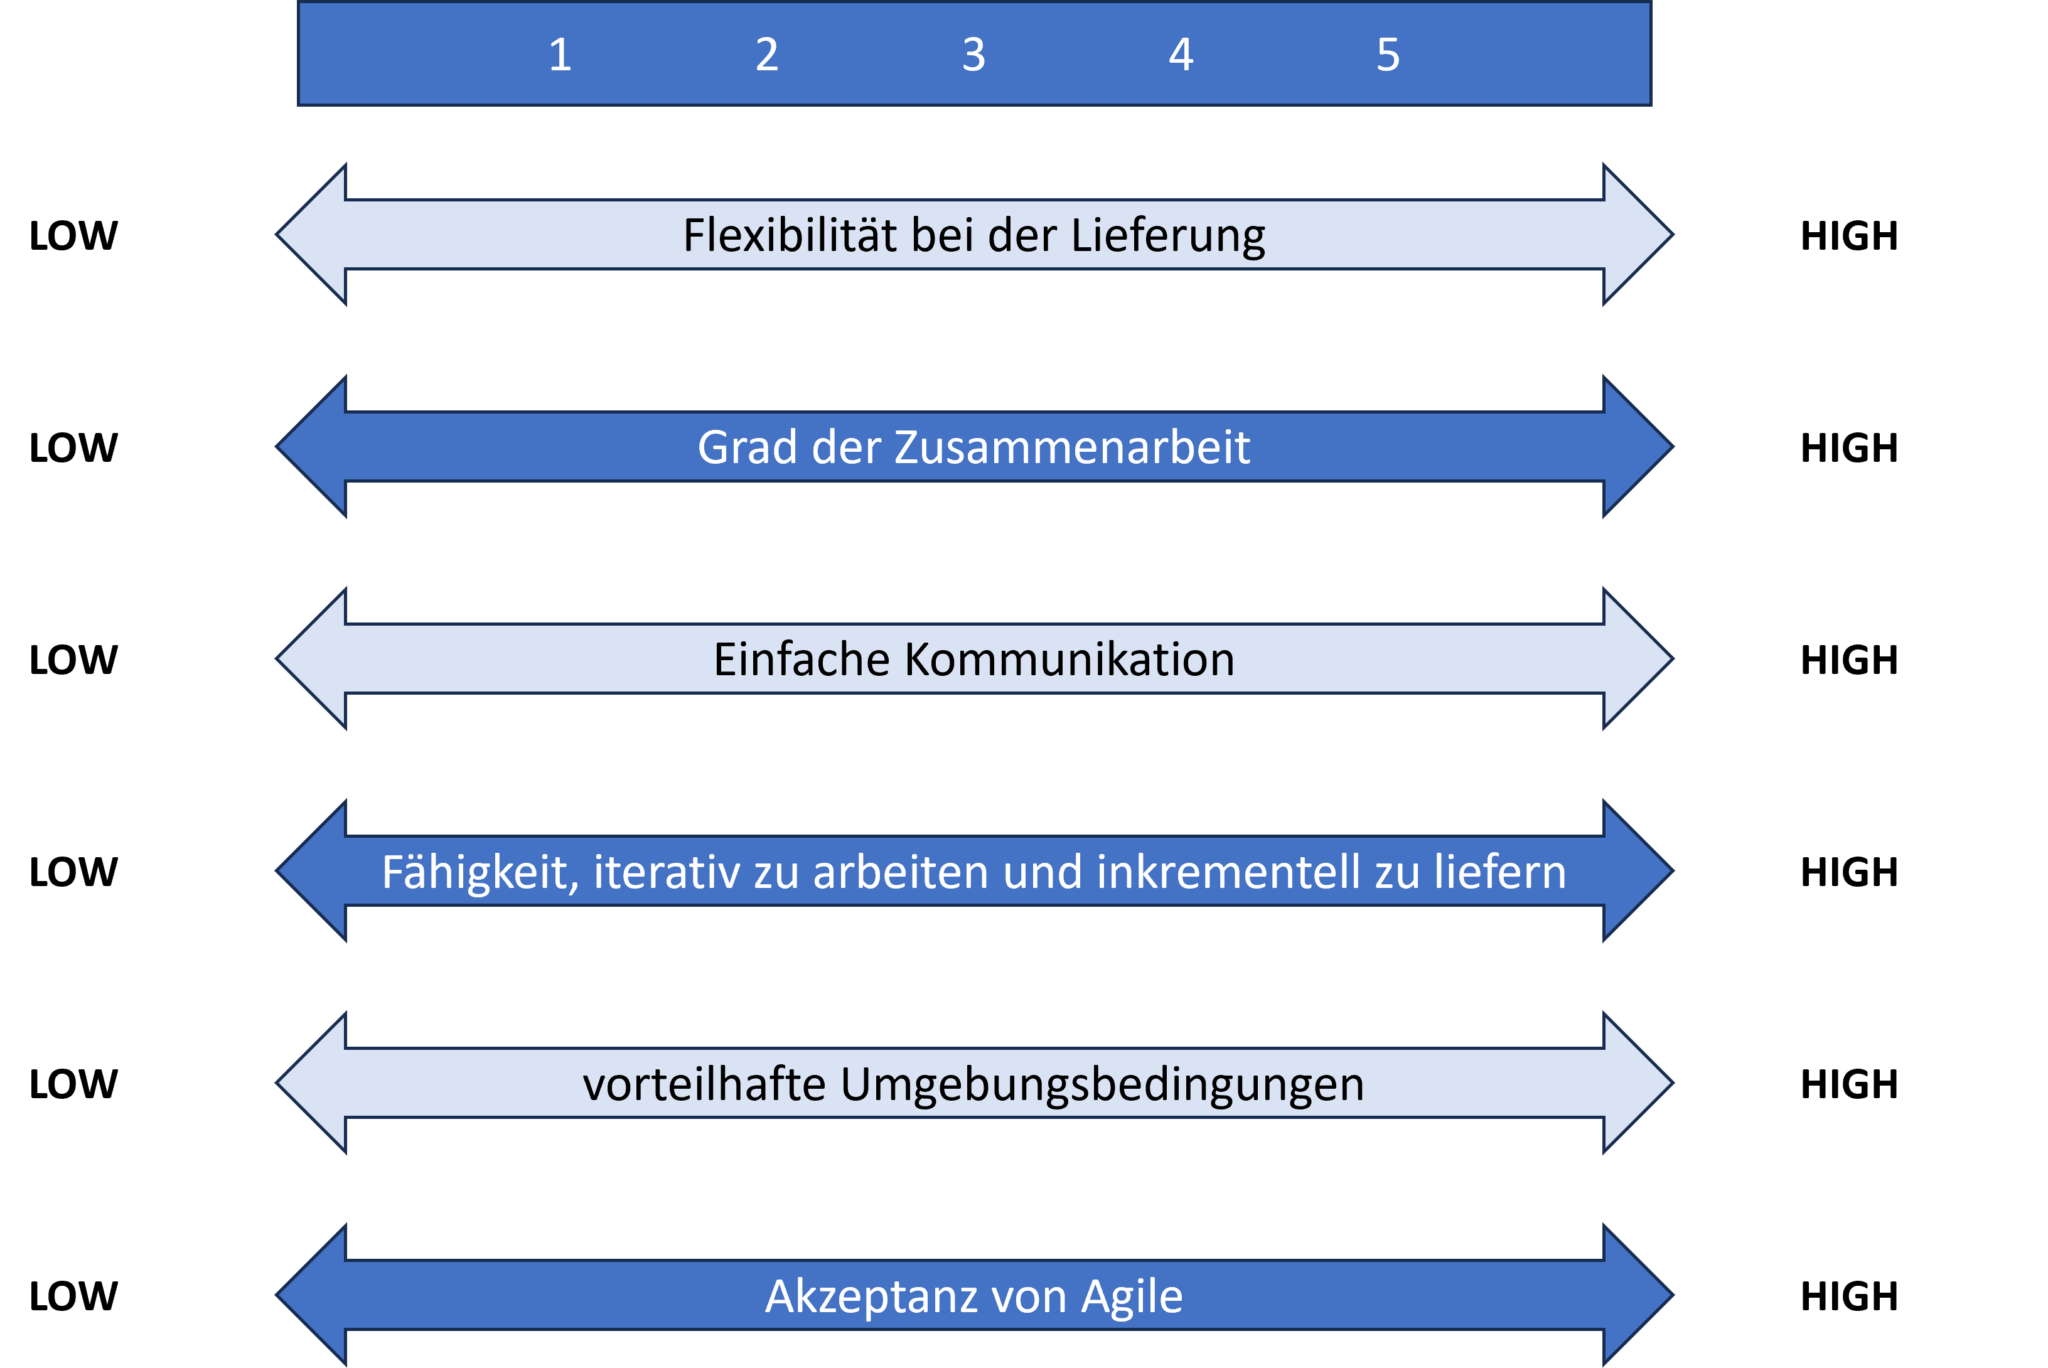
\includegraphics[width=9.69cm, height=6.48cm]{Agilometer}
\caption{Agilometer (\url{https://www.pureconsultant.de/de/agile/agilometer/})}
\end{figure}

Betrachtet man die Philetairus Immobilien GmbH, so ist der agile Reifegrad äußerst niedrig. Es gibt das Bestreben, zumindest auf der für das vorliegende Projekt relevanten Ebene agiler zu agieren, doch die mangelnde praktische Erfahrung bei der umsetzung von agilen Projekten, die immer noch bestehende Skepsis der Unternehmensführung und die große Anzahl von neuen Mitarbeitern in der ausführenden Abteilung deuten darauf hin, dass ein rein agiles Vorgehen keine sinnvolle Wahl wäre.\\

Ein klassisches Vorgehen nach dem Wasserfall- oder V-Modell wäre aufgrund der noch recht unkonkreten Zielsetzung des Projektes auch wenig praktikabel, da für diese Vorgehensweise mit Lasten- und Pflichtenheft die Anforderungen möglichst konkret und unmissverständlich formuliert werden müssen, bevor das Projekt initiiert werden kann.\\

Aus diesem Grund ist für das Vorhaben ein Hybrides Vorgehen, welches klassisches und agiles Vorgehen miteinander verbindet ideal. Für das agile Vorgehen fiel die Entscheidung auf Scrum (siehe ~\ref{subsec:agilesVorgehen}), den klassischen Rahmen soll Prince2 bilden.\\

Prince2 gibt klare Vorgaben, wie das Projektmanagementteam strukturiert sein sollte, für die Planung auf der Teamebene gibt es allerdings keine starren Richtlinien. Daher ist es möglich, ein hybrides Vorgehen zu wählen. Im Fall dieses Projekts wurde die Entscheidung für diese diese Variante getroffen: traditionelles Vorgehen auf der Entscheidungsebene und agiles Vorgehen auf der operativen Ebene. Somit bleibt ein großes Maß an Kontrolle erhalten, ohne die Vorteile des agilen Vorgehens zu sehr zu beschneiden.\\

Auf der anderen Seite definiert der Scrum Guide sehr genau die Rollen und Verantwortlichkeiten auf der Teamebene sowie das Vorgehen während der Entwicklung, die genaue Einbindung in die Unternehmensorganisation wird allerdings nicht konkret vorgegeben, somit ergänzen sich die beiden Vorgehensweisen, da es keine Überlappungen gibt, die Änderungen an einem der beiden Vorgehensmodellen nach sich ziehen und Kompromisse erfordern würden.\\

Ein weiterer Vorteil des Hybriden Vorgehens ist, dass gerade bei Prince2 durch die hohe Anzahl an Projektmanagementprodukten der Dokumentation von Erfahrungswerten ein hoher Wert beigemessen wird, die bei einem rein agilen Vorgehen eine untergeordnete Rolle spielt, wie es im bereits im agilen Mainifest niedergeschrieben wurde:\\

\textit{Funktionierende Software mehr als umfassende Dokumentation}\\

Zwar bedeutet das nicht, dass nicht dokumentiert werden sollte, allerdings wird dem einzelnen Inkrementen die in den Sprints erstellt werden ein höherer Stellenwert beigemessen. Das hybride Vorgehen ermöglicht es, diesem Gedanken gerecht zu werden, indem ein Großteil der Dokumentationsarbeit auf die Projektmanagementebene ausgelagert wird, wodurch das Entwicklerteam entlastet wird, aber dennoch eine umfassende Dokumentation der Erfahrungswerte gewährleistet wird.\\